\documentclass[fleqn,10pt]{wlscirep}

\usepackage{graphicx}
\usepackage{grffile}
\usepackage{textcomp}

\newcommand{\secref}[1]{Section~\ref{sec:#1}}
\newcommand{\tabref}[1]{Table~\ref{tab:#1}}
\newcommand{\figref}[1]{Figure~\ref{fig:#1}}

\newcommand{\beginsupplement}{%
        \setcounter{table}{0}
        \renewcommand{\thetable}{S\arabic{table}}%
        \setcounter{figure}{0}
        \renewcommand{\thefigure}{S\arabic{figure}}%
     }

\newcommand{\textapprox}{\raisebox{0.5ex}{\texttildelow}}

\graphicspath{{./images/}}


\title{Non-Parametric Mixture Modeling for Subtyping Tumors and Identifying Robust Expression Signatures}

\author[1,*]{Jacob Pfeil}
\author[1]{Geoff Lyle}
\author[1]{Lauren Sanders}
\author[1]{Katrina Learned}
\author[1]{Ellen Kephart}
\author[1]{Ann Durbin}
\author[1]{Holly Beale}
\author[1]{Olena Morozova}
\author[1]{Sofie Salama}
\author[1]{David Haussler}
\affil[1]{University of California, Santa Cruz, Biomolecular Engineering, Santa Cruz, 95064, United States}

\affil[*]{jpfeil@ucsc.edu}

%\keywords{Keyword1, Keyword2, Keyword3}

% TODO
% Write results 
% - make figure showing a normally distributed gene expression distribution
% - make neuroblastoma MYCN distribution
% Write methods 
% Write discussion
% Write introduction

\begin{abstract}
Precision oncology is changing the way medicine is practiced by incorporating high-throughput genomic analyses and data analytics. The field has focused on genomic variants, but gene expression data is becoming an additional tool for clinicians to improve patient outcomes. Here, we discuss a novel computational approach for identifying gene expression subtypes that may be helpful for future drug development and risk stratification. We apply this approach to synthetic data as well as patient data from the Cancer Genome Atlas Project. \end{abstract}
\begin{document}

\flushbottom
\maketitle
% * <john.hammersley@gmail.com> 2015-02-09T12:07:31.197Z:
%
%  Click the title above to edit the author information and abstract
%
\thispagestyle{empty}


\section*{Introduction}

% The Introduction section, of referenced text\cite{Figueredo:2009dg} expands on the background of the work (some overlap with the Abstract is acceptable). The introduction should not include subheadings.
RNA-Seq and Bioinformatic tools for quantifying gene expression have been well developed, but there is a need for data analysis approaches for synthesizing this information and generating clinically useful hypotheses. Differential expression approaches are established for comparing two groups, but there are not sufficient methods for identifying related subgroups within a disease population in an unsupervised approach. Genomic and transcriptomic analysis of large cancer research projects have identified common themes across patients and cancers, but the long-tail phenomenon makes it difficult to characterize a large subset of patients that do not have more common genomic alterations.

There are in general two major machine learning approaches. Supervised approaches identify important differences across groups but require knowing the labels that isolate these distinct groups. These methods have limited utility in the precision medicine setting where more descriptive labels are not known before the analysis. Unsupervised methods do not require knowing the clusters in the disease group, but may be sensitive to identifying noise that is not correlated with a variable of interest like survival. Many of the unsupervised clustering approaches also require the user to specify the number of clusters beforehand, which is difficult when trying to identify unknown groups of patients. In practice, researchers fit several unsupervised clustering approaches and nominate the best performing model, but this approach is computationally expensive because a large number of clusters may need to be tested. 

Genomic medicine has become an important component of modern cancer therapies and gene expression analysis is on its way to supplementing and enhancing genomic approaches. Gene expression data has been used to cluster patients into therapeutically related groups. The ability to cluster patients across variant

% Overview of field? I really don't want to start with the whole DNA sequencing has become so popular. Let's write an outline first.
Cancer gene expression analysis has traditionally been used to compare the expression between two groups. The heterogeneity of tumor populations warrants an analysis that can identify differences across multiple subtypes with overlapping features. Differentiating expression at this level has been a challenge, so single-sample approaches have become more popular. However, the single-sample approach does not identify structure within a disease population that would improve the analysis of individual patients. 

% TCGA Gene Expression Data

Many researchers have proposed a mixture modeling approach for differential expression analysis, but a mixture modeling approach has not been adopted by the gene expression analysis community (TODO: ADD REFERENCES TO GENE EXPRESSION MIXTURE MODEL PAPERS). One reason for this is the lack of tools to facilitate this type of analysis. These models are difficult to implement and pre-implemented tools are not well designed for cancer gene expression analysis. There has also been an insufficient number of tissue-specific gene expression profiles to differentiate molecular subtypes. However, the work of TCGA, TARGET, and public repositories not make more sophisticated gene expression analyses possible. 

Most genes' expression distribution is approximately normally distributed once normalized using a log transformation \cite{zwiener2014transforming}. 

% Other approaches in the field
% Here I'll talke about the gene set enrichment approaches

% Overview of method
Commonly used gene expression analyses are used to compare two populations or single samples, but methods are needed to find subtypes within a disease population. Supervised learning approaches like linear regression use known categorical information to learn differences between groups, but these methods are not able to detect subtle differences across a disease population without knowing the differences beforehand. Unsupervised methods are needed to subtype diseases, but one of the limitations in an unsupervised approach is that it is often necessary to specify the number of expected groups beforehand, which limits the ability to discover novel subtypes.

The goal of the hydra algorithm is to enrich for genes of interest by removing genes that are unimodally expressed across a disease cohort. Biomarker development requires gene expression distributions that are detectable in noisy gene expression data. Thus, potential biomarkers must be multimodally expressed and we can use this assumption to identify biomarkers for subtyping tumors and identifying novel drug targets. Multimodally expressed genes may be useful for subtyping tumors, but often there is a variable of interest that covaries with an expression distribution. Once the feature space has been reduced to a smaller size, then the analysis become powered to detected coordinated expression by identifying multivariate clusters. This allows the researchers to investigate the correlation of several genes associated with a variable of interest which will lead to robust detection of expression subtypes and robust gene expression signatures.

Hydra is built upon the Bayesian non-parametric python toolbox bnpy \cite{hughes2014bnpy}. The benefit of a non-parametric approach is that the number of clusters does not need to specified because the algorithm is able to infer the number of clusters from the data. The bnpy library provides a flexible set of tools for performing Dirichlet process mixture modeling. Here, we use the Dirichlet process mixture modeling functions to identify multimodally expressed genes in the univariate setting and a bivariate setting if a covariate variable is provided. The bnpy implementation is fast and can scale to tens of thousands of genes.

The input for the hydra approach is a genes by samples matrix. The Dirichlet process mixture model has the property that as the number of samples increases, the number of clusters identified also increases. The first pass of the hydra pipeline is to identify all of the genes that are multimodally expressed and thus a potential biomarker. If a covariate is provided, then the hydra method does a bivariate clustering to identify genes that are differentially expressed and statistically different in the covariate dimension using a Kruskal-Wallis test \cite{mckight2010kruskal}. The goal of this analysis is to identify the genes that have a strong signal and may subtype tumors. The multimodally expressed genes are then assembled into a multivariate mixture modeling analyis to find coordinated expression of genes that subtype tumors. We have found that these expression networks show related biological function and can be used to identify pathway-level expression for subtyping tumors.

%%%%%%%%%%%%%%%%%%%%%%%%%%%%%%%%%%
% Figure describing hydra %
%%%%%%%%%%%%%%%%%%%%%%%%%%%%%%%%%%
\begin{figure}
	\centering
	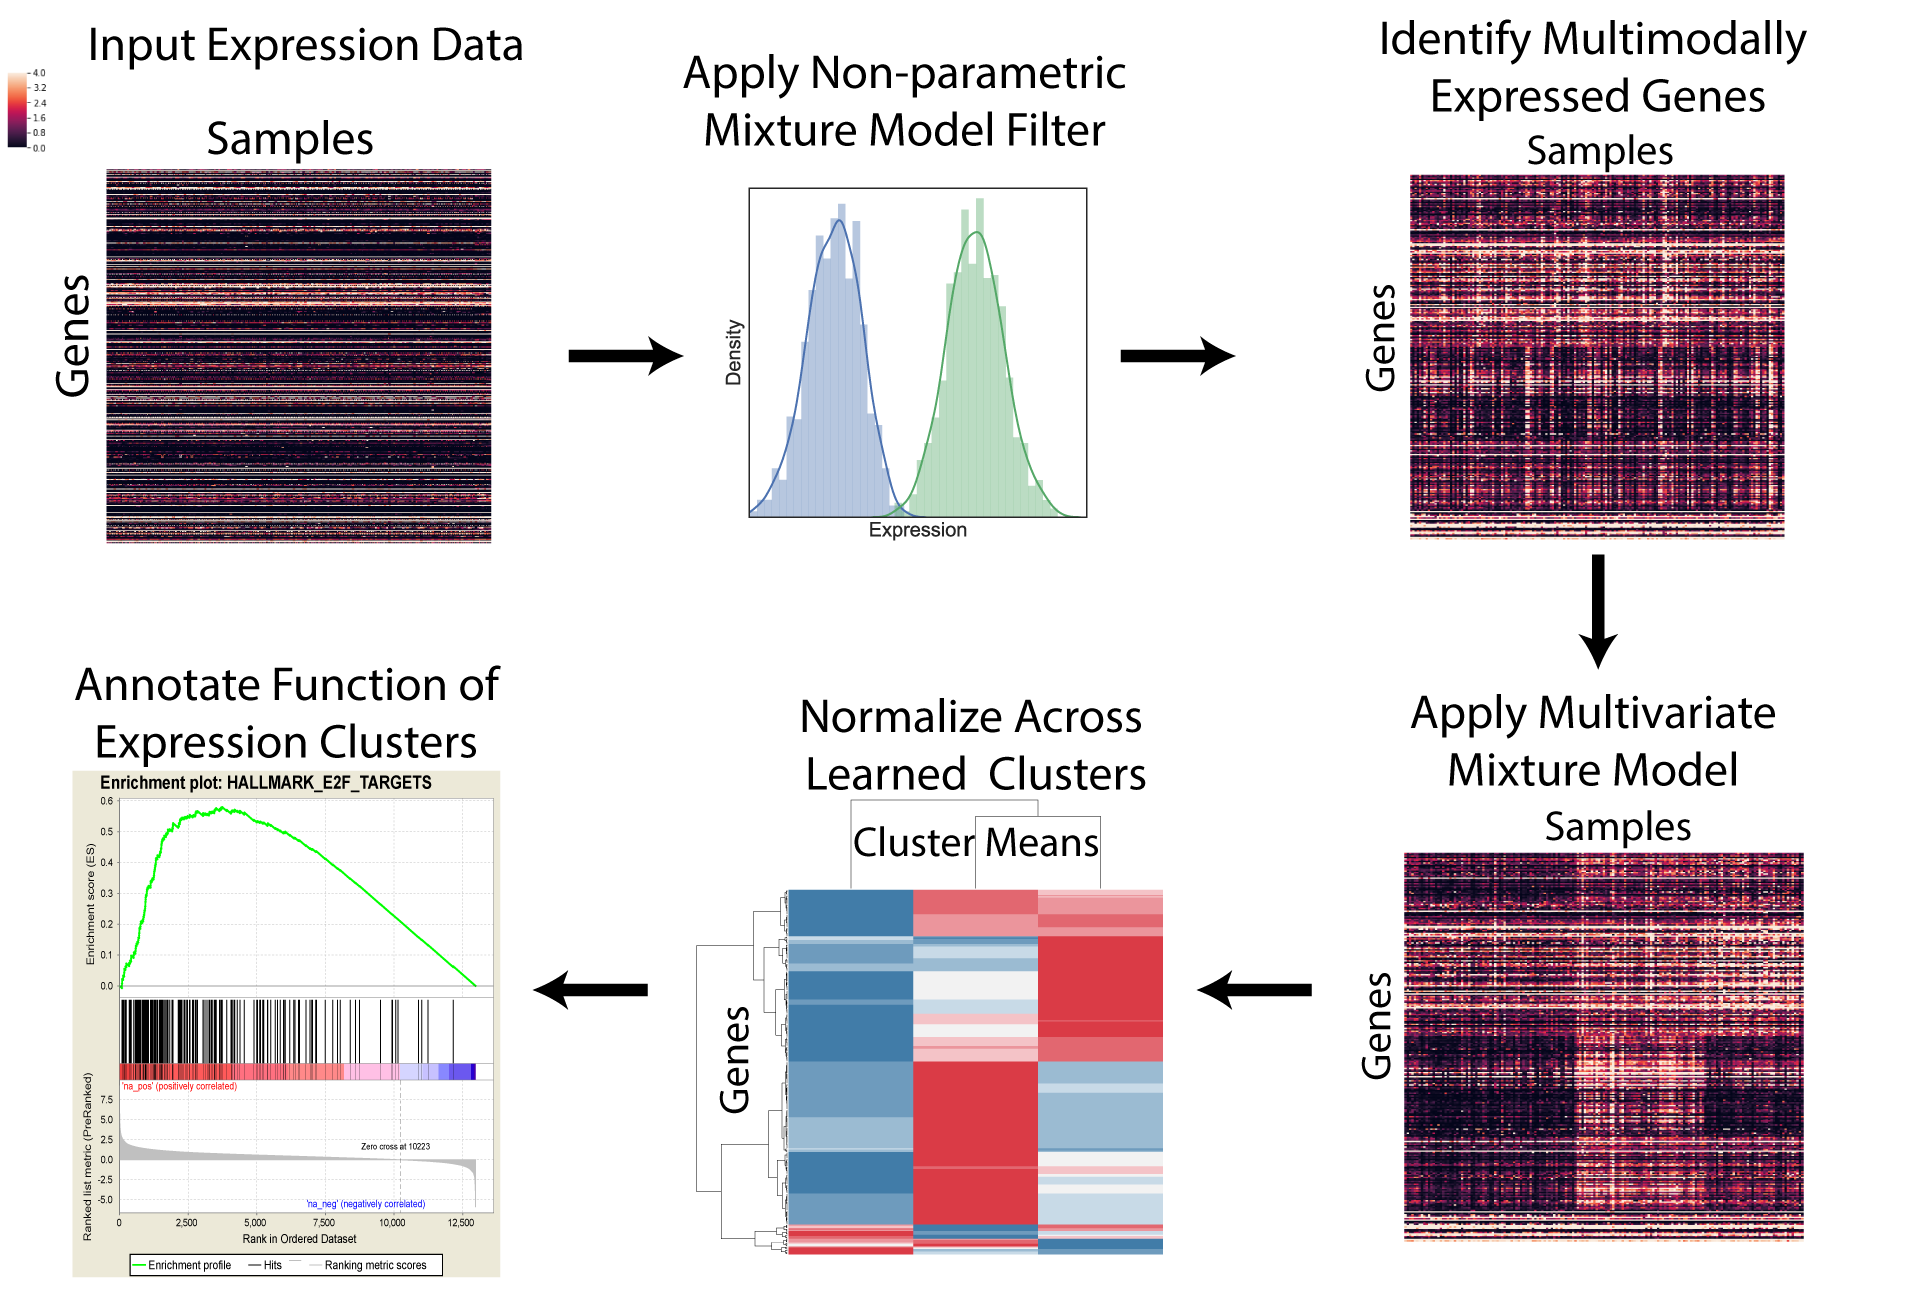
\includegraphics[width=0.75\linewidth]{images/hydra-overview@2x.png}
	\caption{Hydra Method Overview. The hydra pipeline works by taking an input matrix of gene expression profiles across an ideally homogeneous set of samples. The first step in the pipeline is to apply a non-parametric mixture model to learn differentially expressed genes. There is also an option to subset the genes of interest using curated gene sets. Once the multimodally expressed genes are identified, a multivariate mixture model is apply to learn the expression networks that can be used to subtype patients. The parameters are extracted and normalized and the normalized parameters are used to investigate the biological function of gene expression programs using gene set enrichment analysis.}
	\label{sfig:hydra-overview}
\end{figure}

\section*{Method Overview}


\section*{Results}

\subsection*{Synthetic Data Analysis}
Synthetic data was generated to assess the performance of the hydra mixture modeling approach. The synthetic data was generated from GTEx skeletal muscle tissue and randomly assigning a subset of samples to have higher expression for a subset of the MSigDB hallmark genes. We used 26 Hallmark gene sets to simulate activation of a pathway. We created separate synthetic training and test data. We compared our method with single sample gene set enrichment analysis (ssGSEA) \cite{barbie2009systematic} and gene set variation analysis (GSVA) \cite{hanzelmann2013gsva}. These methods are used widely in the field and have been used to identify biological pathway activation and subtype tumors. 

Figure \ref{sfig:rocplot}A highlights two illustrative examples of receiver operator curves with a larger effect size and a smaller effect size with two different gene sets highlighting the influence of background expression in estimating pathway activity.For instance, we compare the performance across these methods for the Hallmark Glycolysis gene set and the Hallmark Oxidative Phosphorylation gene set. The Hallmark Glycoloysis gene set has lower background expression than the Hallmark Oxidative Phosphorylation gene set (TODO: Add mean expression). We found that the ssGSEA method performed comparatively to the hydra method when the background expression is lower, but when the background expression is higher, the ssGSEA method's performance wanes and this effect is related to the effect size. A larger effect size for the change in expression decreases the effect of the background expression.

We next investigated the performance of these methods across 26 Hallmark gene sets (Figure \ref{sfig:rocplot}B). The hydra method performed best across the 26 Hallmark gene sets with a mean of AUC of 0.99 (95\% CI, 0.98 - 1.0 CI). ssGSEA also performed witha mean AUC of 0.93 (95\% CI, 0.90 - 0.96) followed by GSVA with a mean AUC of 0.85 (95\% CI, 0.82 - 0.89).  We also compare the area under the curve from the receiver operator characteristics plot to the mean expression across the Hallmark gene sets and noticed that the ranking methods have lower predictive performance when the background expression for the gene set increases. We found that the background expression for a gene set influenced the performance for ranking methods (Figure \ref{sfig:rocplot}C). Both the GSVA and ssGSEA AUC scores were negatively correlated with the background mean expression level with a Pearson correlation of -0.55 and -0.52, respectively. The hydra approach was not correlated with the background expression levels (p-value $>$ 0.05).

%%%%%%%%%%%%%%%
% ROC Plot Figure %
%%%%%%%%%%%%%%%

\begin{figure}
	\centering
	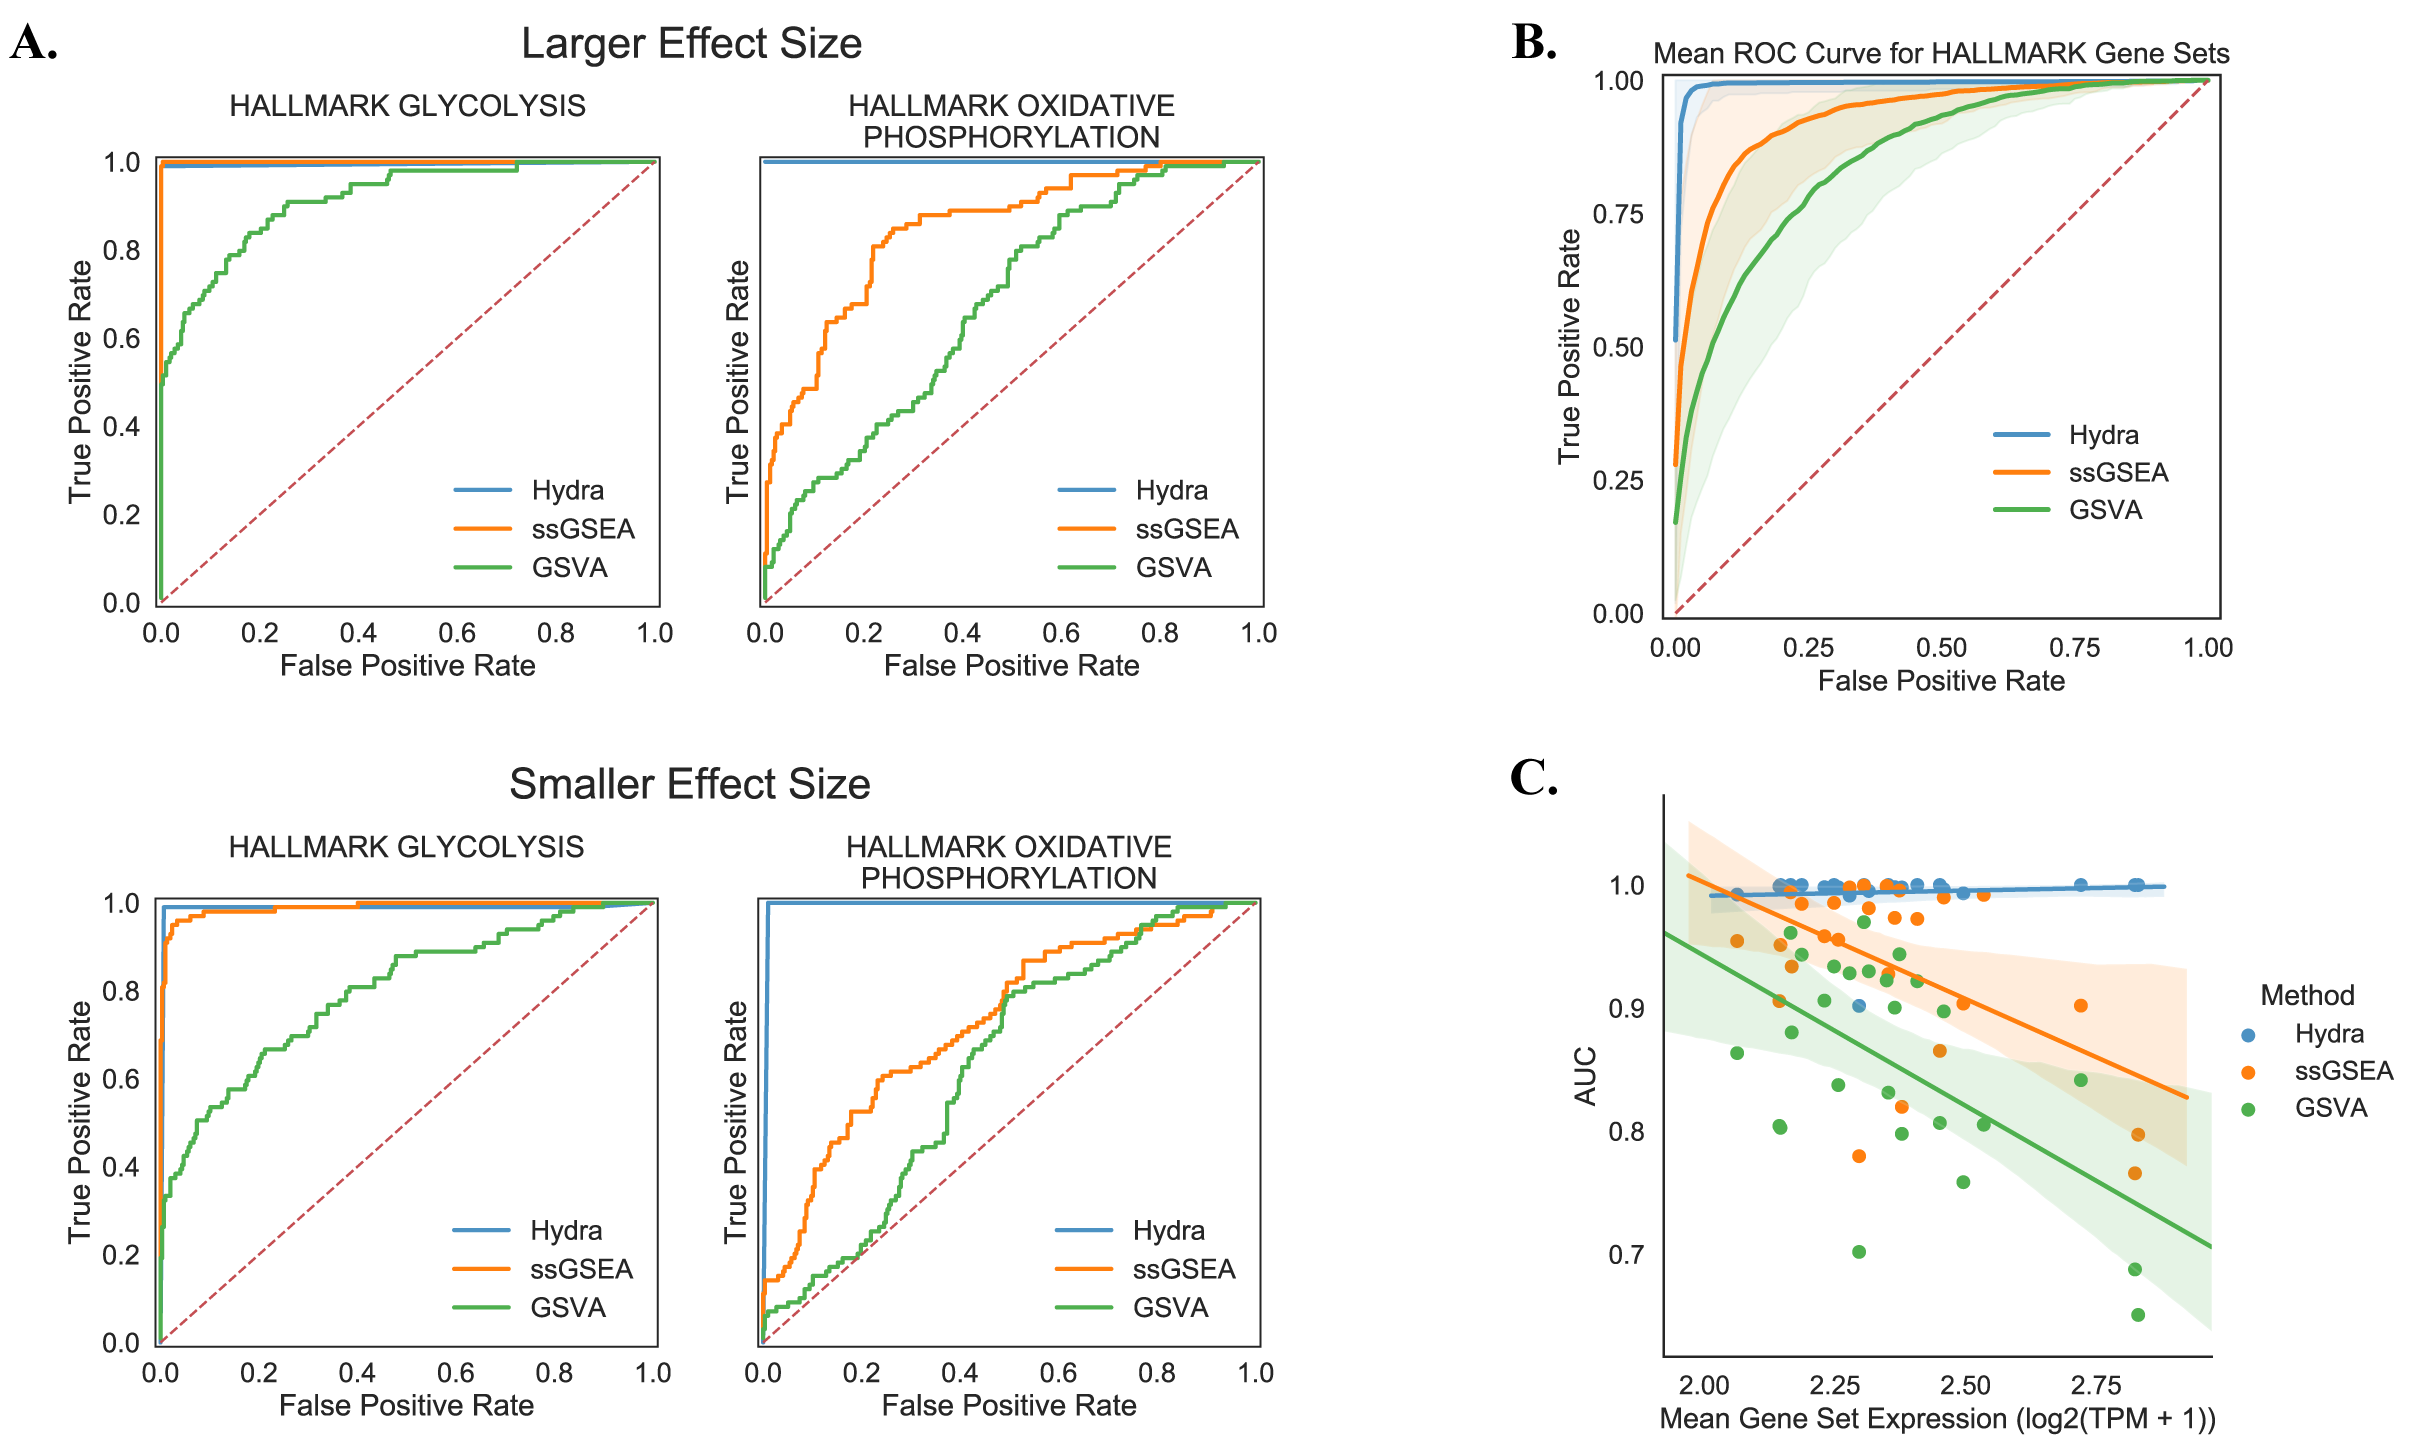
\includegraphics[width=0.8\linewidth]{images/figure-2-roc-curves@2x.png}
	\caption{ROC Plot Curves for Assessing the Performance of Pathway Enrichment Tools.}
	\label{sfig:rocplot}
\end{figure}

\subsection*{Immune Subtype Validation}
The tumor microenvironment plays an important role in providing nutrients and oxygen to the tumor, shielding cancer cells from the immune system, and providing growth factors that promote cancer growth and resistance to therapies \cite{hanahan2012accessories}. We applied the hydra method to identify immune subtypes of melanoma using the TCGA skin cutaneous melanome RNA-Seq data (N=383) hosted on the Xena browser \cite{vivian2017toil}. We used the IMMPORT database to identify immune subtypes in the TCGA melanoma data set \cite{bhattacharya2018immport}. We set a minimum mean expression value for a gene to 1 log2(TPM + 1). The IMMPORT gene list started with 1,740 genes and identified 570 genes that are multimodally expressed. The multivariate clustering algorithm identified 8 clusters. Hierarchical clustering using the Ward method across the mean expression levels across clusters identified three major subtypes of melanoma (Figure \ref{sfig:melanoma}A). We next compared the estimated leukocyte infiltrate as determined by Saltz et al. (2018) \cite{saltz2018spatial}. The hydra approach identified statistically different immune infiltrates by the nonparametric Kruskal-Wallis test (p $<$ 0.01).

We next compared the hydra subtype identification clusters to another published method for enumerating cell types within gene expression data known as CIBERSORT \cite{newman2015robust}. Lymphocytes, MAST cells, and macrophages were differentially abundant in the TCGA melanoma tissue samples (Kruskal-Wallis p $<$ 0.01) (Figure \ref{sfig:melanoma}C). Clusters 6, 0, and 5 have elevated lymphocyte expression but lower Mast cell and macrophage associated expression (TODO: Add statistical test). Subtypes 2, 1, 3, 4, 7 have subtype had higher total leukocyte infiltration with cluster 5 having the highest estimate of leukocyte infiltrate.


%%%%%%%%%%%%%%%%%%%%%%%%%%%%%%
% SKCM Immune Subtype Figure %
%%%%%%%%%2%%%%%%%%%%%%%%%%%%%%%

\begin{figure}
	\centering
	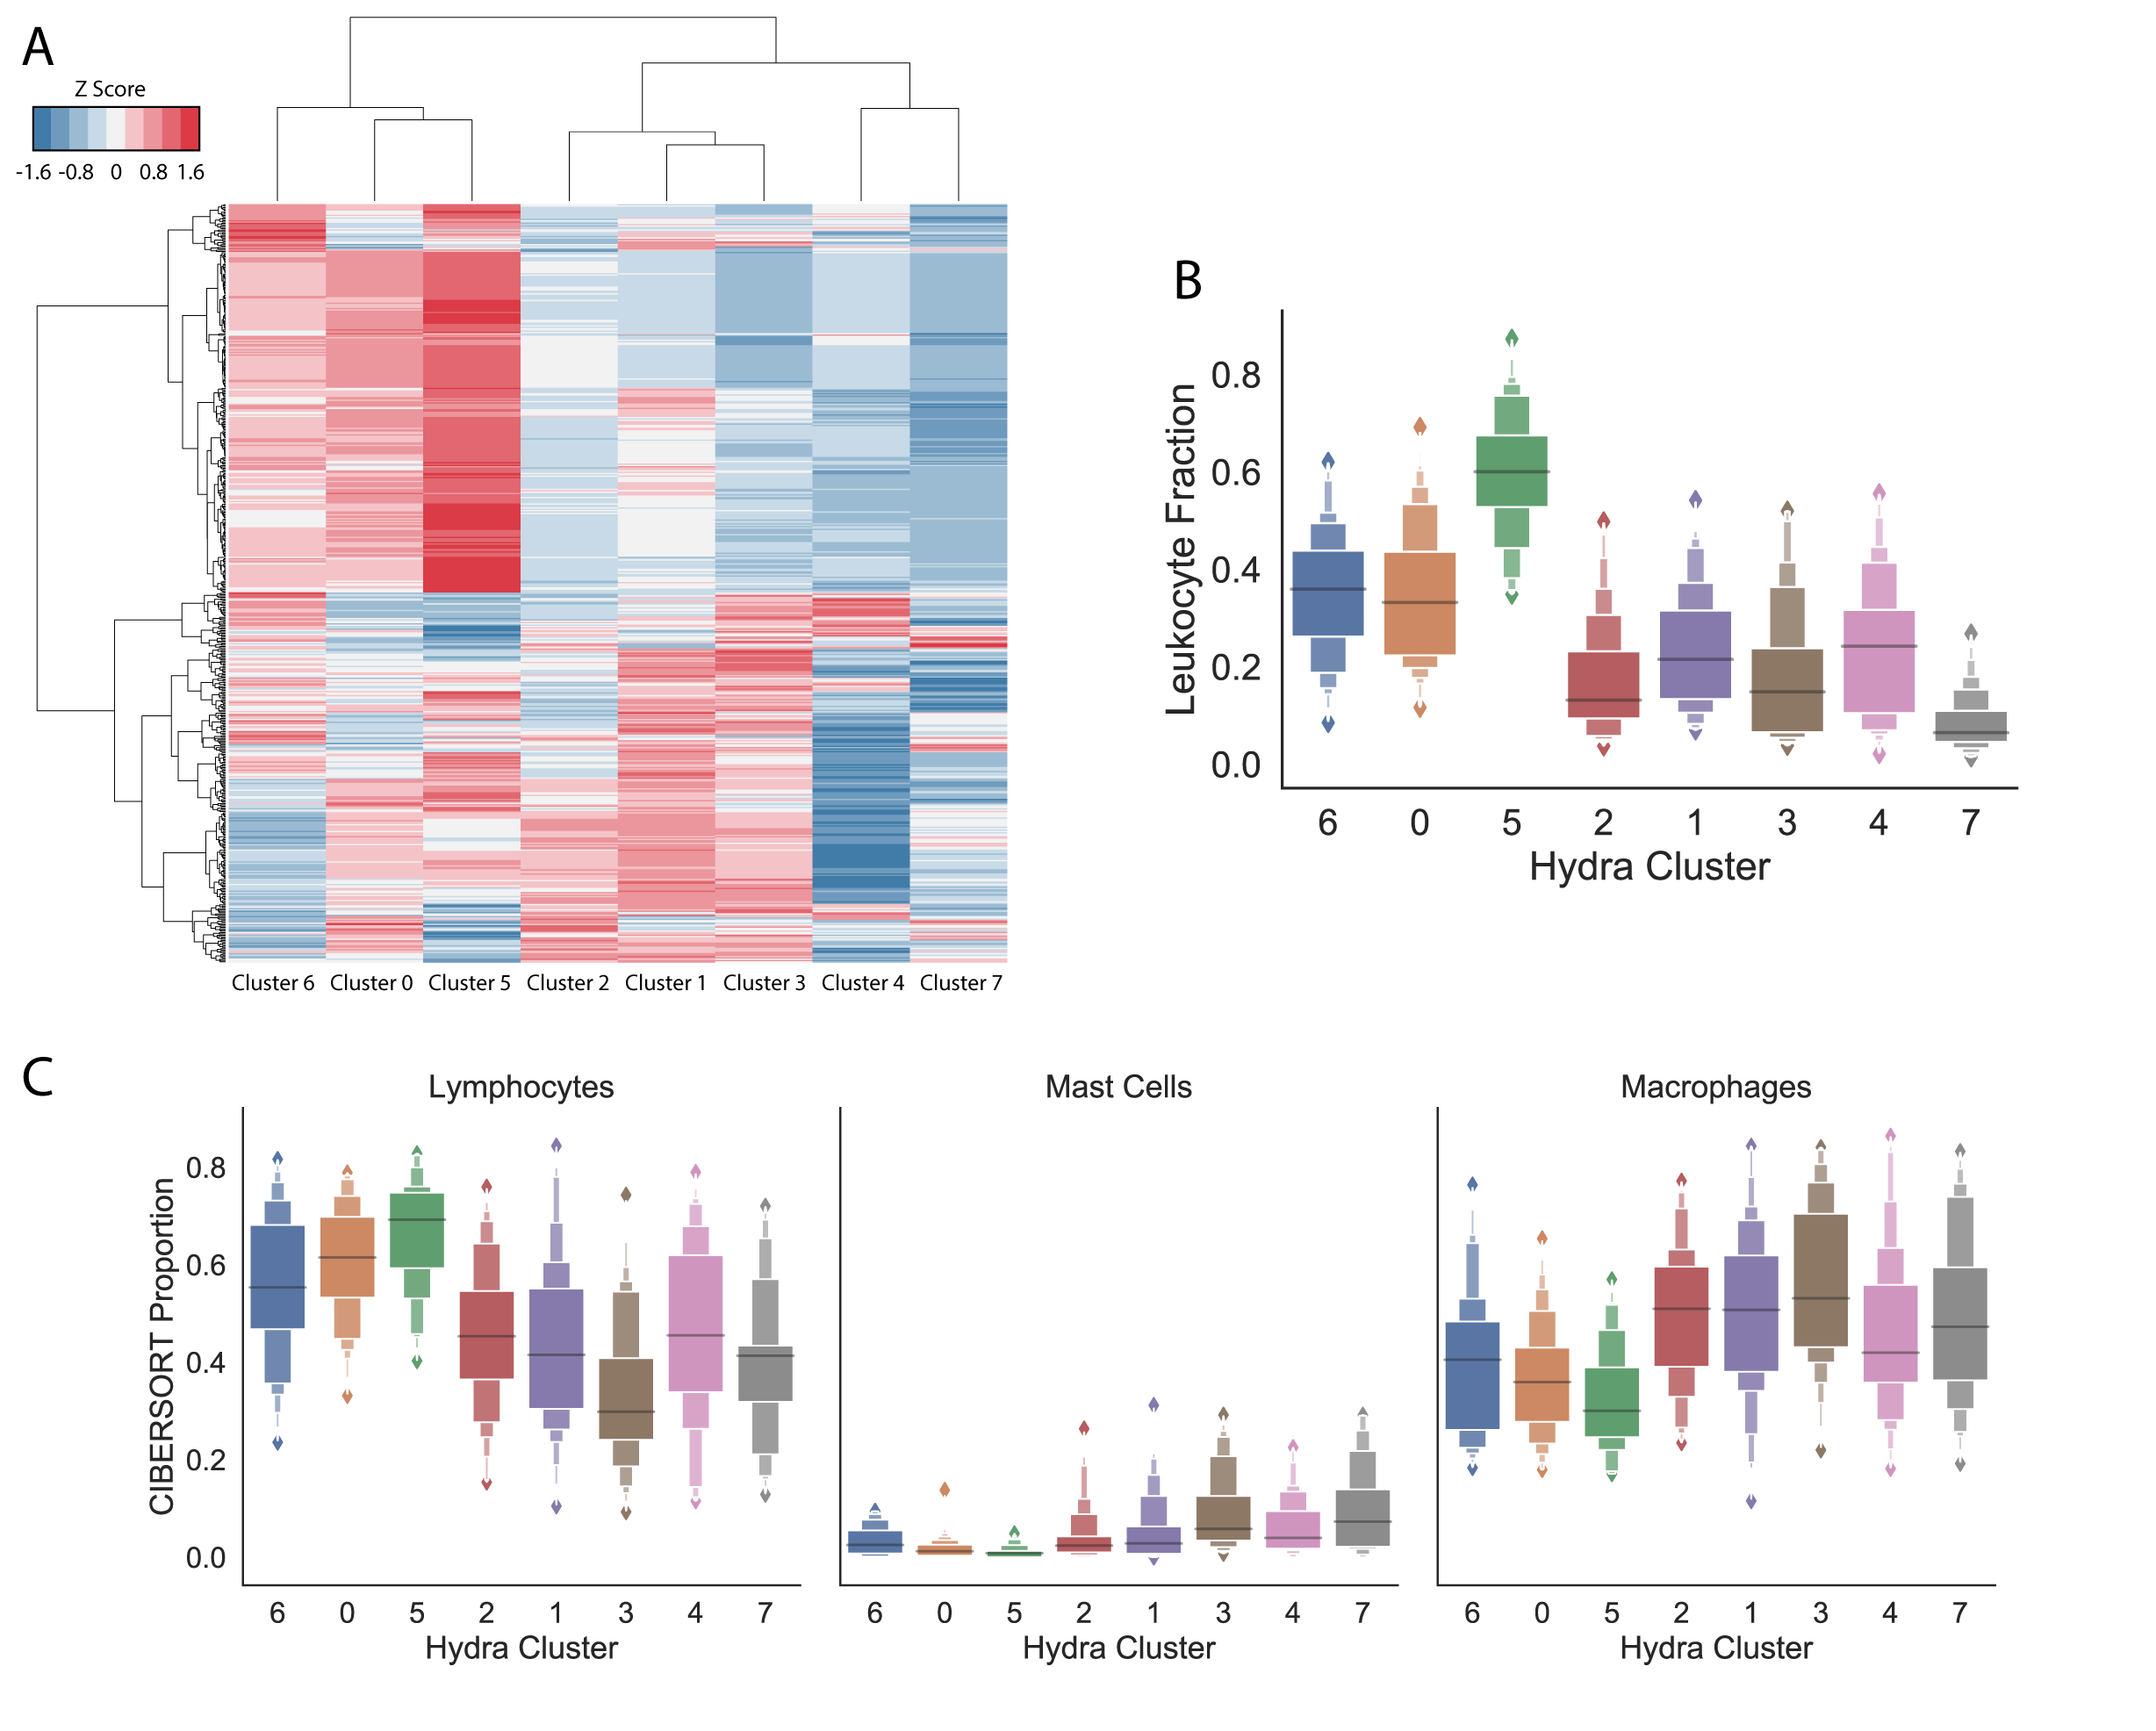
\includegraphics[width=0.75\linewidth]{images/melanoma-immune-subtypes-immport-boxen@2x.png}
	\caption{Melanoma Immune Subtyping and Validation. The hydra clustering algorithm identified 8 melanoma subtypes. Comparing these subtypes to a whole-slide image analysis of H\&E slides identified statistically significant differences in the leukocyte infiltrate across the hydra clusters (B). Further analysis of the clusters using the CIBSORT algorithm identified statistically significant differences for the lymphocyte, Mast cell, and macrophage expression (C). TODO: Make another figure where the immune cell expression is interspersed into one plot so show the contrast in immune infiltrate.}
	\label{sfig:melanoma}
\end{figure}

%%%%%%%%%%%%%%%%%%%%%%%%%%%%%%%
% SKCM Immune Survival Figure %
%%%%%%%%%2%%%%%%%%%%%%%%%%%%%%%

\begin{figure}
	\centering
	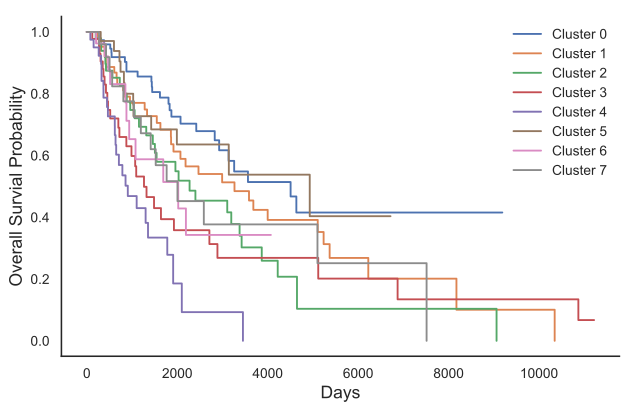
\includegraphics[width=0.75\linewidth]{images/immport-skcm-cluster-survival.png}
	\caption{Hydra Subtypes Predict Poor Survival in Melanoma.}
	\label{sfig:melanoma-surv}
\end{figure}


We next investigated the survival for different immune clusters and identified a survival benefit from a high lymphocyte to macrophage ratio. For example, cluster six grouped with the elevated lymphocyte fraction and had a statistically significant improvement in survival compared to a cluster that had lower immune infiltrate and a higher macrophage fraction (Figures \ref{sfig:melanoma} and \ref{sfig:melanoma-surv}). Gene set enrichment analysis for the subtypes that had a statistically significant survival benefit were also enriched for T-cell infiltrate whereas cluster 4 was not enriched for an immune gene set suggesting that the cancer cells were unchecked by the immune system . 

% Need a paragraph about the TCGA immune subtype paper




\subsection*{Molecular Subtype Validation}
Gene expression analysis is also used to identify molecular subtypes of cancer. Genetic and epigenetic alterations lead to changes in expression and these changes can be quantified using RNA-Seq technology and compared across patients to find molecular subtypes.


%%%%%%%%%%%%%%%%%%%%%%
% TCGA BRCA Subtypes %
%%%%%%%%%%%%%%%%%%%%%%
\begin{figure}
	\centering
	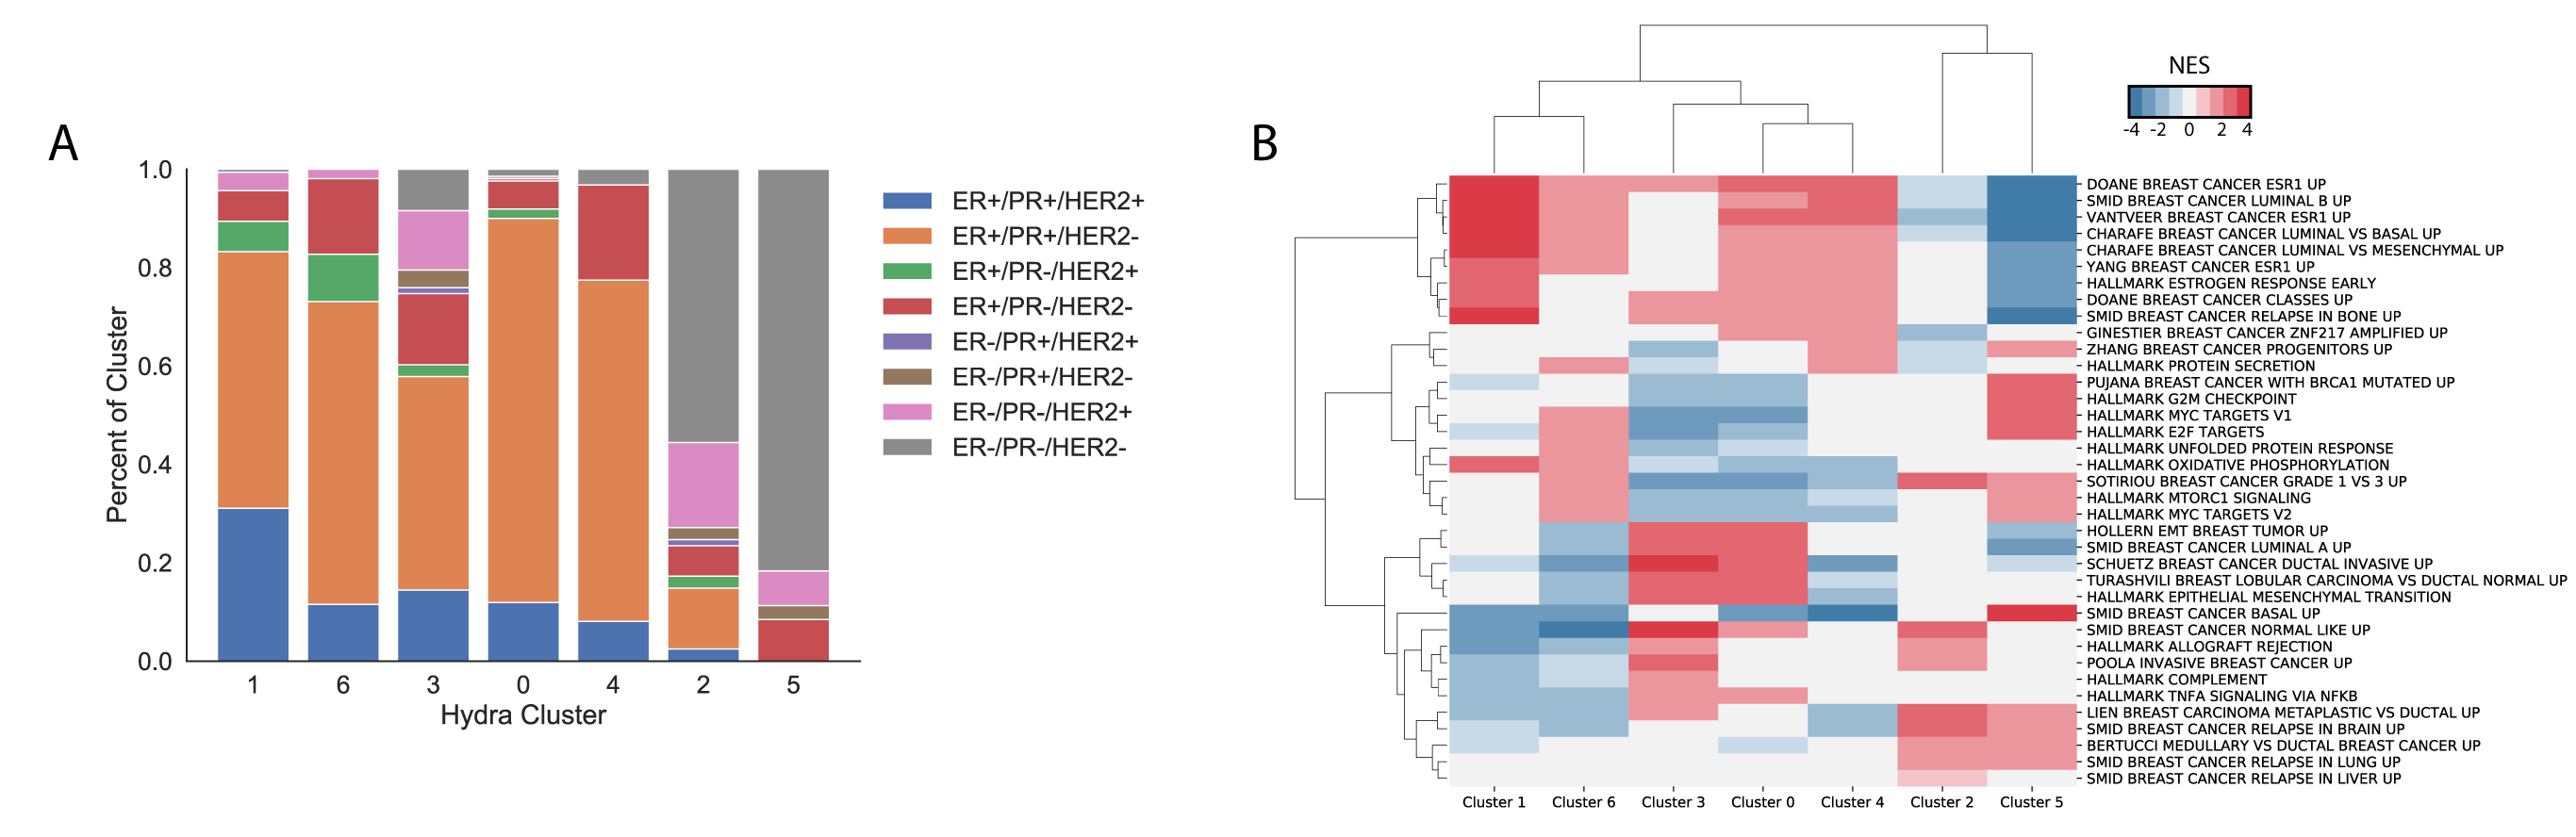
\includegraphics[width=1.1\linewidth]{images/tcga-brca-subtyping-figure@2x.png}
	\caption{Hydra Subtypes Identify Known Breast Cancer Subtypes.}
	\label{sfig:brca-subtypes}
\end{figure}


\begin{figure}
	\centering
	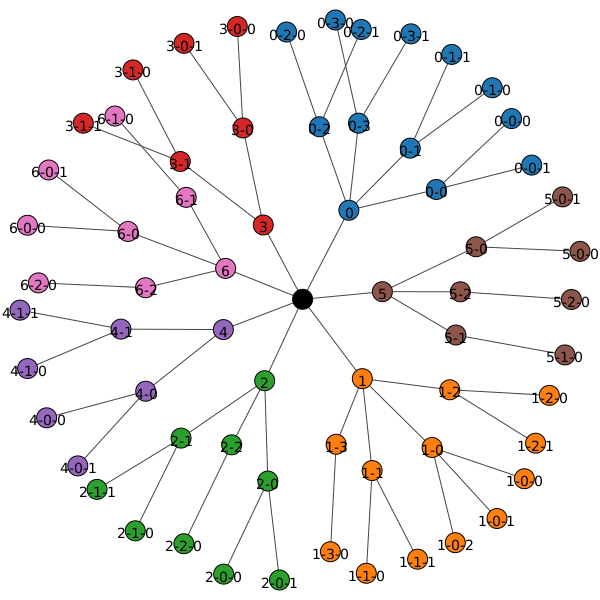
\includegraphics[width=0.8\linewidth]{images/tcga-brca-subcluster-tree.png}
	\caption{Iterative clustering reveals hidden structure within TCGA BRCA data. }
	\label{sfig:brca-ihydra}
\end{figure}

\begin{figure}
	\centering
	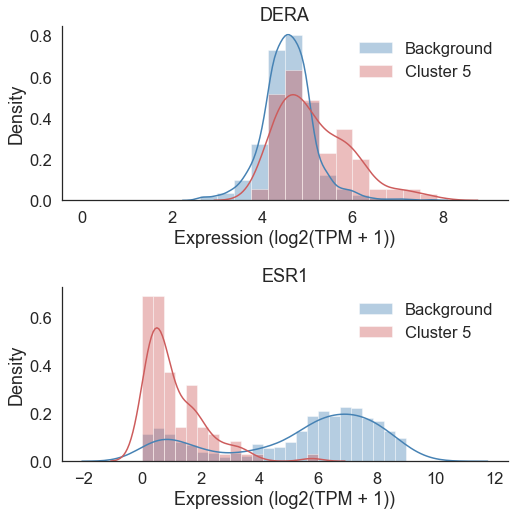
\includegraphics[width=0.75\linewidth]{images/example-subtyping-distribution-changes.png}
	\caption{Iterative clustering reveals hidden structure within TCGA BRCA data. }
	\label{sfig:brca-expression-subtypes}
\end{figure}


\begin{table}
\begin{tabular}{clcc}
	\toprule
	{} &                                         Gene Set &   NES & P-Value \\
	Cluster &                                                  &       &         \\
	\midrule
	0       &                SMID BREAST CANCER NORMAL LIKE UP &  3.08 &   0.002 \\
	0       &                  SMID BREAST CANCER LUMINAL A UP &  2.23 &   0.008 \\
	1       &                      SMID BREAST CANCER BASAL UP &  3.78 &   0.044 \\
	2       &                      SMID BREAST CANCER BASAL UP &  2.29 &   0.003 \\
	2       &               ZHANG BREAST CANCER PROGENITORS UP &  1.82 &   0.037 \\
	3       &                      DOANE BREAST CANCER ESR1 UP &  3.82 &   0.001 \\
	3       &                  SMID BREAST CANCER LUMINAL B UP &  3.19 &   0.001 \\
	3       &                   DOANE BREAST CANCER CLASSES UP &  3.12 &   0.001 \\
	3       &        CHARAFE BREAST CANCER LUMINAL VS BASAL UP &  3.09 &   0.001 \\
	3       &  CHARAFE BREAST CANCER LUMINAL VS MESENCHYMAL UP &  3.08 &   0.001 \\
	3       &            SMID BREAST CANCER RELAPSE IN BONE UP &  3.08 &   0.001 \\
	3       &                      SMID BREAST CANCER ERBB2 UP &  2.70 &   0.001 \\
	3       &                       YANG BREAST CANCER ESR1 UP &  2.61 &   0.001 \\
	3       &                   VANTVEER BREAST CANCER ESR1 UP &  2.49 &   0.001 \\
	3       &                  SMID BREAST CANCER LUMINAL A UP &  1.95 &   0.021 \\
	\bottomrule
\end{tabular}
	\caption{TCGA Triple Negative Breast Cancer Subtypes}
	\label{stab:tnbc-table}
\end{table}

\section*{Discussion}

The Discussion should be succinct and must not contain subheadings.

One of the benefits of this approach is that this provides a framework for understanding a population of patients and can identify subtypes that may benefit from future drug development. Investigation into subtype specific expression may also identify opportunities to repurpose available therapies for other diseases. This is particularly useful for pediatric cancer gene expression analysis where drug development has lagged and there is a need for novel therapies. 

One of the limitations of a non-parametric ranking approach to gene set enrichment is that it cannot account for the dynamic range in expression for a gene in a single-sample context. Therefore, we hypothesized that a GSEA method approach that does not account for this information will suffer if the background expression for a gene set is high. We see this in the HALLMARK Oxidative Phosphorylation analysis where the ssGSEA suffers from poor performance because the background expression is higher and thus is not well suited to identify subtle changes in expression.


\section*{Methods}

%Topical subheadings are allowed. Authors must ensure that their Methods section includes adequate experimental and characterization data necessary for others in the field to reproduce their work.

\subsection{Synthetic Data Generation}
The MSigDB Hallmark gene sets were used to simulate biological pathway expression that reflects the gene set properties of a typical gene expression analysis \cite{liberzon2015molecular,liberzon2011molecular}. We also needed a large cohort of human tissue samples to infer differentially expressed genes. We used the GTEx skeletal muscle cohort \cite{consortium2013genotype}. To simulate subtype specific expression, we randomly sampled 25\% of the patient population and then we sampled from a normal distribution centered at 0.5 with a standard deviation of 0.5. We then added this value to 25\% of the genes in each Hallmark gene set to simulate coordinated expression of genes within a biological gene set.

We compared the predictive performance for identifying enriched genes using healthy tissue samples collected as part of the Genotype-Tissue Expression (GTEx) project \cite{lonsdale2013genotype}. The Molecular Signatures Database (MSigDB) provides a large set of curated gene lists for identifying biological functions for precision medicine applications. We used the Hallmark MSigDB gene sets to select genes with related biological functions and correlated expression \cite{liberzon2015molecular}. We then randomly sampled GTEx skeletal muscle samples, modified their expression values for a subset of the gene set genes. We did this process twice to generate synthetic training and test data. The same genes were used in the test and training data, but the values were sampled independently from a normal distribution at varying mean differences. 

We applied this analysis to all of the Hallmark gene sets, but we are showing two illustrative examples here (TODO: add figure ref). The Hallmark Glycolysis gene set includes 199 genes involved in glycolysis and gluconeogenesis. We sample 25\% of these genes to be differentially expressed and sampled a difference in expression value from a normal $\mathcal{N}(0.5, 0.5)$ or a $\mathcal{N}(1, 0.5)$. If this difference caused a negative expression value, then we set the expression value to be zero. The GTEx expression TPM values were generated using the Toil RNA-Seq pipeline \cite{vivian2017toil}. The reciever operator curves (ROC) were generated for the hydra, ssGSEA, and GSVA methods. The hydra method performed the best with an AUC (area under the curve) of X, but the ssGSEA method was comparable with an AUC of blank. The GSVA method performed the worst with an AUC of BLANK.



\bibliography{reference}

\section*{Acknowledgements (not compulsory)}

Acknowledgements should be brief, and should not include thanks to anonymous referees and editors, or effusive comments. Grant or contribution numbers may be acknowledged.

\section*{Author contributions statement}

J.P. conceived the analysis, conducted the analysis, and wrote the paper. O.M., H.B., S.S., and D.H. reviewed the results and contributed feedback. All authors reviewed the manuscript. 

\section*{Additional information}

To include, in this order: \textbf{Accession codes} (where applicable); \textbf{Competing financial interests} (mandatory statement). 

The corresponding author is responsible for submitting a \href{http://www.nature.com/srep/policies/index.html#competing}{competing financial interests statement} on behalf of all authors of the paper. This statement must be included in the submitted article file.

\beginsupplement
\section*{Supplementary Information}

\subsection*{Cancer Gene Expression Distributions are Multi-Modal}
\subsubsection*{Modes Correspond to Sex-Specific Expression}
Genes are expressed at different levels for different tissues. In addition to tissue specific expression, there are also biological features that influence gene expression across individuals. For example, age and gender are correlated with expression of some genes. A varying effects model where the mean and the effect of biological features change depending on the tissue can be used to make better predictions of gene expression. For example, a hierarchical model can identify sex-linked expression, but the current pan-cancer and pan-disease analyses are not able to detect sex-linked expression. An example of sex-linked expression that has been associated with cancer is the XIST gene \cite{yildirim2013xist}. XIST controls X-chromosome silencing in females and is not usually expressed in males (\figref{xist}). This is a clear example where assuming male and female gene expression comes from the same distribution leads to an exaggerated estimation of the outlier threshold. It is therefore difficult to identify potential cases where under-expression of XIST in females may contribute to their cancer. While the incidence of cancer is equal across boys and girls, boys tend to respond worse to therapy. An investigation into sex-linked gene expression may yield insights into the differences in response to cancer therapies for boys and girls. 

%%%%%%%%%%%%%%%
% XIST Figure %
%%%%%%%%%%%%%%%

\begin{figure}
\centering
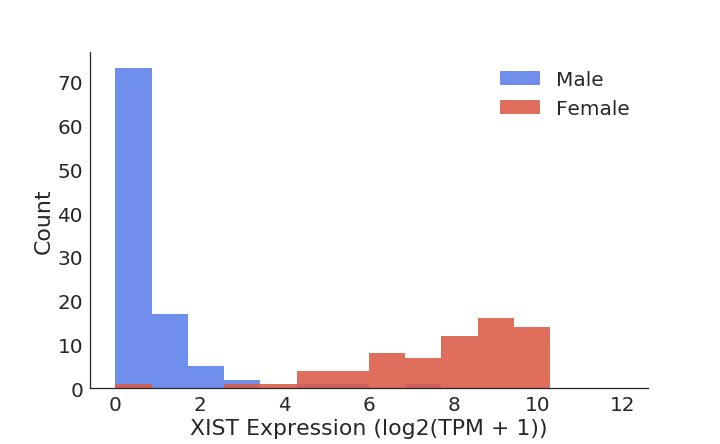
\includegraphics[width=0.75\linewidth]{images/xist-fig-2017-12-28.png}
\caption{Example of gender-specific expression that can be modeled in a hierarchical model. The XIST gene is involved in X chromosome silencing, so XIST is not expressed for males. XIST has been linked to cancer, but the Treehouse model overestimates the variance in XIST expression because females and males are modeled together. The proposed hierarchical model learns the differences between male and female XIST expression for improved model fit.}
\label{sfig:xist}
\end{figure}


%%%%%%%%%%%%%%%%%%%%%%%%%%
% MYCN Validation Figure %
%%%%%%%%%%%%%%%%%%%%%%%%%%

\begin{figure}
	\centering
	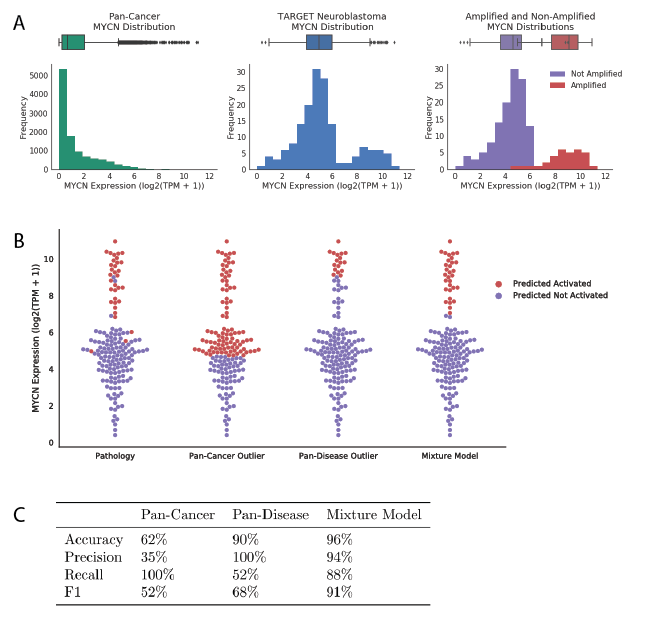
\includegraphics[width=0.75\linewidth]{images/MYCN-Figure.png}
	\caption{MYCN Validation}
	\label{sfig:mycn}
\end{figure}

%%%%%%%%%%%%%%%%%%%%%%%%%%%%%%%%
% Melanoma Gene Set Enrichment %
%%%%%%%%%%%%%%%%%%%%%%%%%%%%%%%%

\begin{figure}
	\centering
	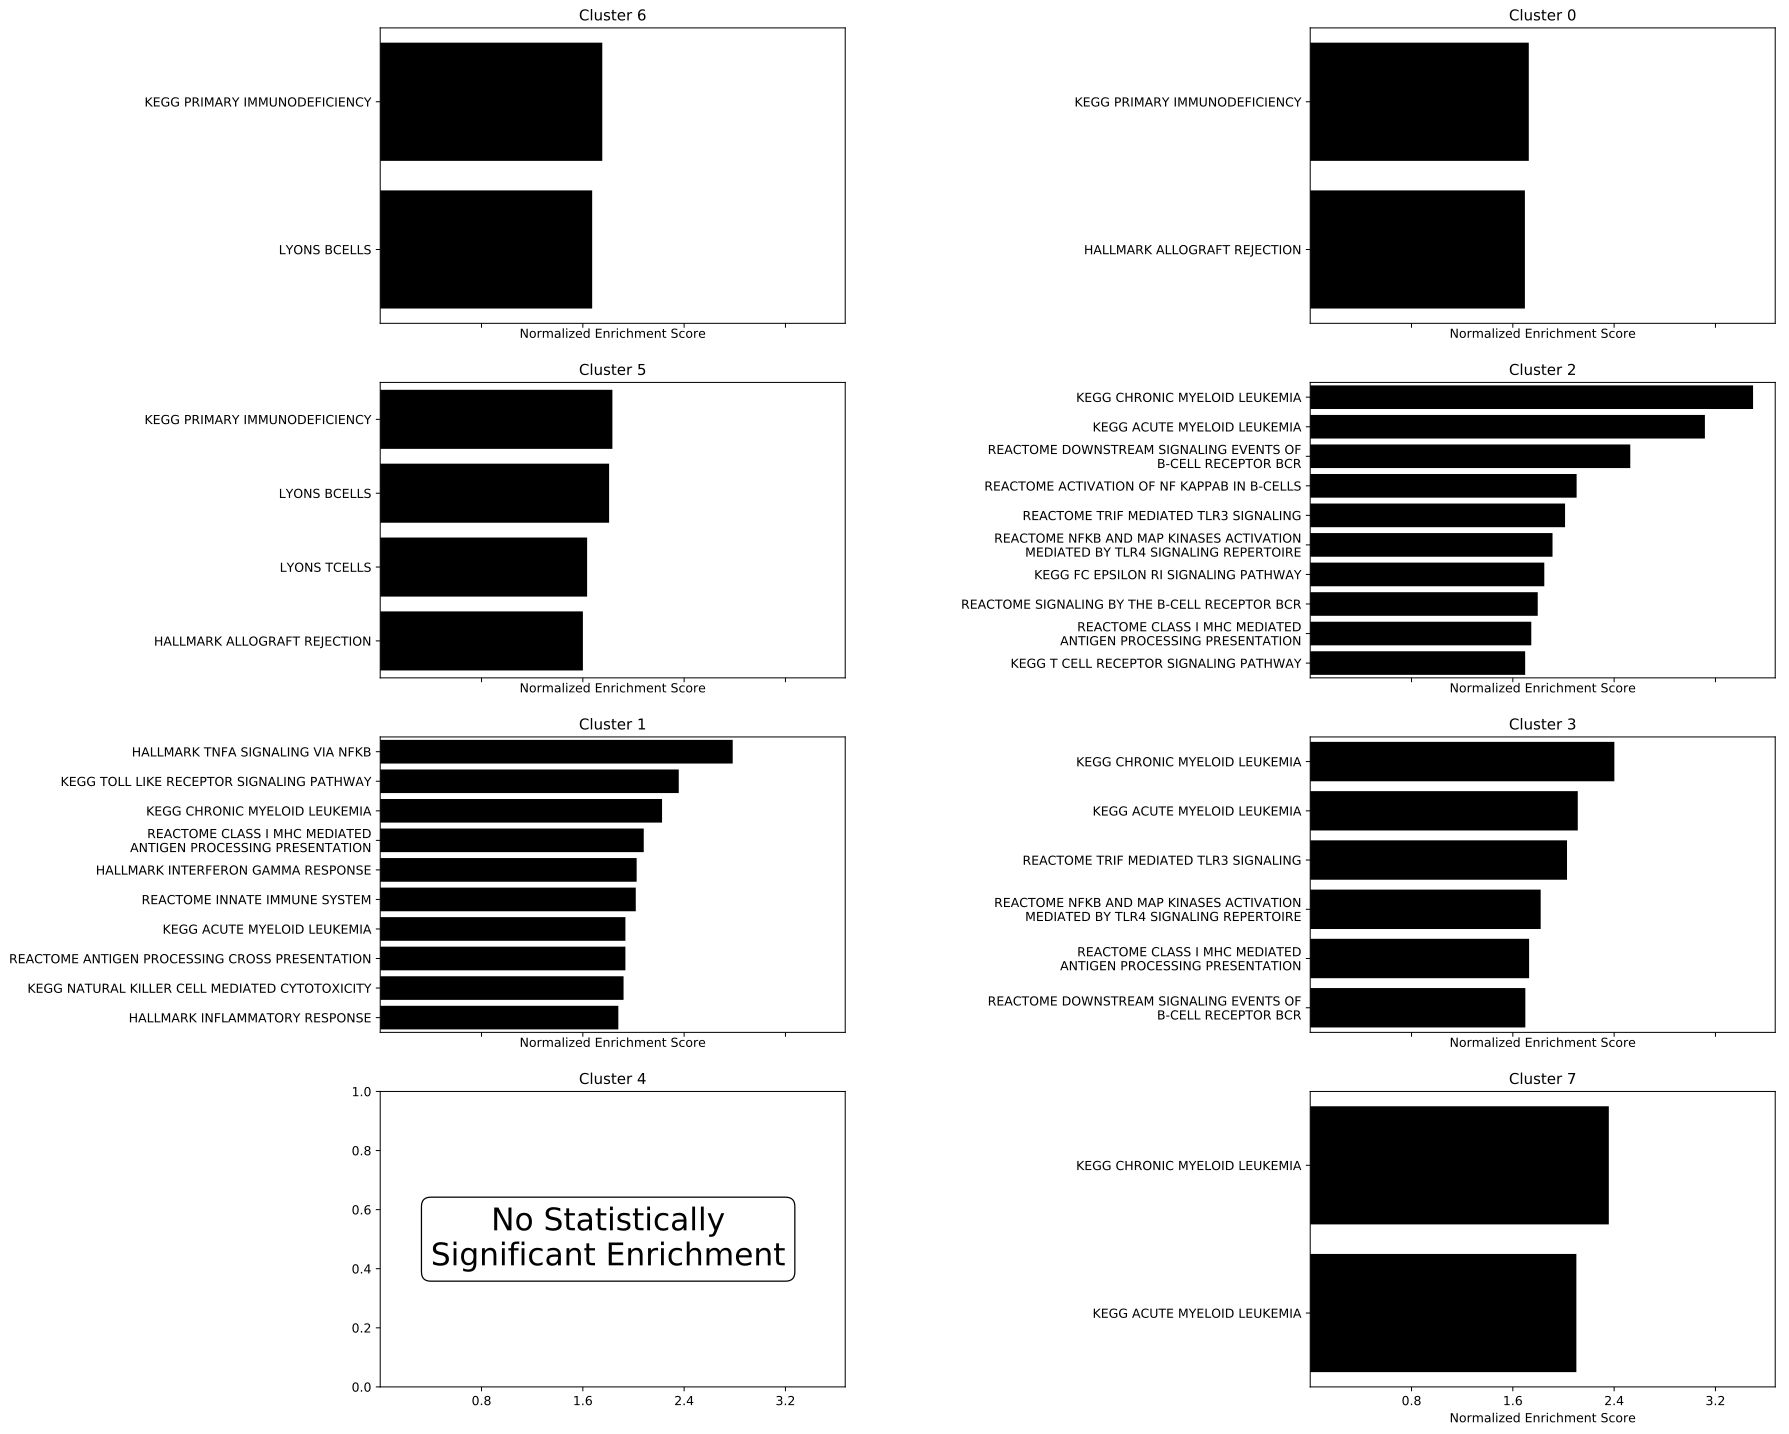
\includegraphics[width=0.75\linewidth]{images/melanoma-immune-subtype-enrichment.png}
	\caption{Melanoma Cluster Immune Gene Set Enrichment}
	\label{sfig:melanoma-gsea}
\end{figure}




\end{document}